\documentclass{ltjsarticle}
\usepackage[version=4]{mhchem} % 化学記法用パッケージ
\usepackage{amsmath}         % 数式拡張用
\usepackage{chemfig}         % 必要に応じた反応機構図の描画用
\usepackage{tikz}            % TikZ (3D描画等のため)
\usepackage[dvipdfmx]{pict2e}  % picture環境の拡張（古い環境の場合は epic/eepic の読み込みも検討）

% --- picture環境による構造式描画用定義 ---
% 横向きベンゼン環 \benzene
\def\benzene{{\unitlength.1pt%
\raisebox{-7pt}{\begin{picture}(223,195)%
  \linethickness{.5pt}%
  \font\tenln=linew10%
  \put(0,96){\line(10,17){56}}%
  \put(54,191){\line(1,0){114}}%
  \put(166,191){\line(10,-17){56}}%
  \put(0,98){\line(10,-17){56}}%
  \put(54,5){\line(1,0){114}}%
  \put(166,5){\line(10,17){56}}%
  \put(23,98){\line(10,17){45}}%
  \put(155,173){\line(10,-17){45}}%
  \put(66,22){\line(1,0){90}}%
\end{picture}}}}

% 横向きフェニル基 \phenyl
\def\phenyl{{\unitlength.1pt%
\raisebox{-7pt}{\begin{picture}(301,195)%
  \linethickness{.5pt}%
  \font\tenln=linew10%
  \put(0,96){\line(10,17){56}}%
  \put(54,191){\line(1,0){114}}%
  \put(166,191){\line(10,-17){56}}%
  \put(0,98){\line(10,-17){56}}%
  \put(54,5){\line(1,0){114}}%
  \put(166,5){\line(10,17){56}}%
  \put(23,98){\line(10,17){45}}%
  \put(155,173){\line(10,-17){45}}%
  \put(66,22){\line(1,0){90}}%
  \put(220,98){\line(1,0){80}}%
\end{picture}}}}

% 横向きベンゼンパラ二置換体 \para
\def\para{{\unitlength.1pt%
\raisebox{-7pt}{\begin{picture}(378,195)%
  \linethickness{.5pt}%
  \font\tenln=linew10%
  \put(77,96){\line(100,173){57}}%
  \put(132,192){\line(1,0){113}}%
  \put(243,192){\line(100,-173){56}}%
  \put(77,98){\line(10,-17){57}}%
  \put(132,3){\line(1,0){113}}%
  \put(243,3){\line(100,173){56}}%
  \put(100,98){\line(100,173){45}}%
  \put(232,173){\line(100,-173){45}}%
  \put(143,22){\line(1,0){90}}%
  \put(297,98){\line(1,0){80}}%
  \put(0,98){\line(1,0){80}}%
\end{picture}}}}

% オルト・メタ二置換体の定義
\makeatletter
% オルト二置換体：\ortho{置換基1}{置換基2}
\def\ortho#1#2{{\unitlength.1pt%
\raisebox{-7pt}{\begin{picture}(270,225)%
  \linethickness{.5pt}%
  \font\tenln=linew10%
  \put(2,56){\line(0,1){113}}%
  \put(2,167){\line(173,100){97}}%
  \put(2,58){\line(173,-100){95}}%
  \put(96,2){\line(173,100){97}}%
  \put(192,56){\line(0,1){113}}%
  \put(97,222){\line(173,-100){97}}%
  \put(22,157){\line(173,100){76}}%
  \put(22,68){\line(173,-100){76}}%
  \put(173,69){\line(0,1){87}}%
  \put(192,167){\line(173,100){76}}%
  \put(192,57){\line(173,-100){76}}%
\end{picture}}%
\nobreak\kern2pt\nobreak
\setbox0\hbox{\raisebox{12pt}{\ce{#1}}}%
\setbox1\hbox{\raisebox{-9pt}{\ce{#2}}}%
\ifdim\wd0>\wd1 \@tempdima=\wd0\else \@tempdima=\wd1\fi
\nobreak\makebox[0pt][l]{\usebox0}\nobreak\makebox[\@tempdima][l]{\usebox1}}}

% メタ二置換体：\meta{置換基1}{置換基2}
\def\meta#1#2{{\unitlength.1pt%
\raisebox{-7pt}{\begin{picture}(270,310)%
  \linethickness{.5pt}%
  \font\tenln=linew10%
  \put(2,56){\line(0,1){113}}%
  \put(2,167){\line(173,100){97}}%
  \put(2,58){\line(173,-100){95}}%
  \put(96,2){\line(173,100){97}}%
  \put(192,56){\line(0,1){113}}%
  \put(97,222){\line(173,-100){97}}%
  \put(22,157){\line(173,100){76}}%
  \put(22,68){\line(173,-100){76}}%
  \put(173,69){\line(0,1){87}}%
  \put(192,57){\line(173,-100){76}}%
  \put(97,220){\line(0,1){89}}%
\end{picture}}%
\nobreak\kern2pt\nobreak
\setbox0\hbox{\kern-23pt\raisebox{26pt}{\ce{#1}}}%
\setbox1\hbox{\raisebox{-9pt}{\ce{#2}}}%
\ifdim\wd0>\wd1 \@tempdima=\wd0\else \@tempdima=\wd1\fi
\nobreak\makebox[0pt][l]{\usebox0}\nobreak\makebox[\@tempdima][l]{\usebox1}}}
\makeatother
% --- ここまで picture環境による描画用定義 ---

\begin{document}

\title{化学記法の新たな視点：\TeX による表現技法の探究}
\author{Example Researcher}
\maketitle

\section{序論}
本稿では、\texttt{mhchem}パッケージを中心とした基本記法に加え、分子の立体配置、反応条件、電子移動、同位体ラベリング、多核錯体、そしてポリマー化学に至るまで、化学記法の多様な側面を取り上げる。さらに、任意の化合物の記述や複雑な立体構造の視覚化に関する拡張記法についても考察する。これらの記法の正確性は、実験再現性や理論解析の厳密化に寄与するのみならず、分子間相互作用や反応機構の解釈をより深いものとする。

\section{基本の分子式記述}
\verb|\ce| コマンドにより、以下のような基本的な分子式が直感的に記述できる：
\begin{itemize}
  \item 水：\ce{H2O}
  \item 二酸化炭素：\ce{CO2}
  \item グルコース：\ce{C6H12O6}
\end{itemize}
これらは分子構造の抽象化と実験データとの対応を支える基本的要素である。

\section{化学反応式の記述}
反応経路の明示は、実験および理論の双方において不可欠である。例えば、
\[
\ce{2H2 + O2 -> 2H2O}
\]
や、平衡反応を示す場合は
\[
\ce{CO + H2O <=> CO2 + H2}
\]
と記述される。

\section{特殊な化学種の表記}
錯体やイオンなど、複雑な化学種も \verb|\ce| コマンドにより容易に表記可能である。例として、
\[
\ce{[Ag(CN)2]^-}, \quad \ce{Na+}, \quad \ce{Cl-}
\]
などが挙げられる。

\section{立体化学の表現}
分子の三次元構造は、その反応性や相互作用に大きな影響を与える。鏡像異性体の識別には \ce{(R)-} や \ce{(S)-} の表記が用いられ、ウェッジ・ダッシュ記法により立体配置を明示する手法が確立されている。これにより、分子内部の空間的な配置がどのように化学反応に影響するかが、より精密に示される。

\section{反応条件および触媒の記述}
温度、圧力、溶媒、さらには触媒といった反応条件は、反応の進行や選択性に直接影響を及ぼす。これらの条件は、矢印の上下に併記することで次のように表現される：
\[
\ce{A ->[heat][catalyst] B}
\]
この記法は、実験条件を正確に伝え、再現性の高い記述を可能とする。

\section{反応機構と電子移動の記述}
単一の反応式では捉えきれない電子の移動や中間体の生成は、曲線矢印を用いた記法で補完される。例えば、\texttt{chemfig}パッケージを活用すれば、以下のような反応機構図を描画できる：
\[
\chemfig{A -[0.5,0.5]B}
\]
この手法により、反応経路の詳細な解析および電子の流れが視覚的に示され、理論計算の精度向上に寄与する。

\section{同位体及び放射性元素の表記}
分子動態解析や反応経路の追跡には、同位体ラベリングが不可欠である。\ce{^13C}、\ce{^{18}O}といった表記により、特定の原子種の挙動を詳細に追跡することが可能となる。また、放射性元素に関しては、原子番号や質量数を明確に示す記法が求められる。

\section{複雑な配位化学と多核錯体の記法}
単一の錯体表記に留まらず、配位数や幾何学的配置、多核錯体といった複雑な系の記述も現代化学では重要なテーマである。各原子間の結合関係や錯体内部の電子分布を適切に表現するため、記法の拡張が不可欠であり、これが理論解析および応用研究の信頼性向上に直結する。

\section{ポリマー記法の応用例}
ポリマー化学では、繰り返し単位や分子量の指標が特に重要である。繰り返し構造は
\[
\ce{(C2H4)_n}
\]
のように表記され、架橋構造や分岐構造も併せて記述することで、物理的性質や機能性の詳細な解析が可能となる。

\section{多様な立体化学の表記法}
任意の化合物の立体配置を正確に記述するため、以下の表記法も重要である。

\subsection{E/Z および cis/trans 表記}
二重結合の配置を示すために、E/Z 表記が用いられる。例えば、
\[
\ce{RCH=CH{R'}}
\quad (\text{EまたはZ})
\]
と表記する（ここでは、アポストロフィーを中括弧で囲むことでエラーを回避している）。また、環状構造では cis/trans 表記が適用される。
  
\subsection{Newman 投影}
分子内の回転異性体を示すためには、Newman 投影が有用である。以下はエタンの回転異性体を概念的に示す例である：
\begin{center}
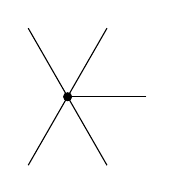
\begin{tikzpicture}[scale=1.0]
  % 中心の炭素原子を示す点
  \draw[fill=black] (0,0) circle (0.05cm);
  % 前面の結合（実線）
  \draw (-0.5,0.87) -- (0,0);
  \draw (0.5,0.87) -- (0,0);
  \draw (1,0) -- (0,0);
  \draw (0.5,-0.87) -- (0,0);
  \draw (-0.5,-0.87) -- (0,0);
\end{tikzpicture}
\end{center}

\subsection{Fischer 投影}
特に糖類やアミノ酸の立体配置を示す際に用いられる。例えば、グルコースは以下のように表記できる：
\[
\ce{HOCH2(CHOH)_{4}CHO}
\]
この記法により、各炭素の配置が直感的に理解できる。

\section{拡張的な構造式記法}
複雑な有機化合物の記述には、線式（Line-Angle式）や縮約式（Condensed式）も有用である。例えば、ベンゼンは線式では六角形として描かれ、縮約式では
\[
\ce{C6H6}
\]
と表記される。また、SMILES記法のような文字列ベースの表記法は、デジタルデータとして広く利用されている。

\section{3次元構造の描画技法の拡充}
Chemfigパッケージに加え、TikZやPGFPlotsの3D描画機能を活用することで、分子の立体配置や反応経路をより精密に描画できる。たとえば、TikZの3Dライブラリを利用した場合の例は以下の通りである：
\begin{verbatim}
\begin{tikzpicture}[tdplot_main_coords]
  % ここに3D分子描画のコード例を記述
\end{tikzpicture}
\end{verbatim}
これにより、分子の空間配置やエネルギー面、反応経路の3次元的表現が可能となる。

\section{特殊な化合物の記法}
多核錯体や複雑な配位化学の系については、各中心の配位環境や架橋構造を明確に示す必要がある。例えば、以下のような記法が考えられる：
\[
\ce{[M_2L_4]^{n+}}
\]
ここで、Mは金属中心、Lは配位子を表す。さらに、各結合角や配位数について詳細に記述することで、反応機構や電子分布の解析に寄与する。

% ===== 新章：picture 環境による構造式描画とその応用 =====
\section{picture 環境によるベンゼン環等の描画と応用例}
本章では、picture 環境を用いて横向きのベンゼン環やその派生図形（フェニル基、パラ二置換体、オルト・メタ二置換体）を描画する方法と、\verb|\ce| コマンドと組み合わせた反応式表現の一例を示す。

\subsection{定義済み図形}
前述の定義により、以下の図形が利用可能である：
\begin{itemize}
  \item 横向きベンゼン環：\verb|\benzene|
  \item 横向きフェニル基：\verb|\phenyl|
  \item 横向きベンゼンパラ二置換体：\verb|\para|
  \item オルト二置換体：\verb|\ortho{置換基1}{置換基2}|
  \item メタ二置換体：\verb|\meta{置換基1}{置換基2}|
\end{itemize}

\subsection{使用例}
以下は、\verb|\ce| コマンドと組み合わせた使用例である。
\begin{verbatim}
\ce{{\benzene} + HNO3 ->C[~~\Delta~~][] {\phenyl} NO2 + H2O}

\ce{{\phenyl} NH2 + NaNO2 + 2HCl -> {\phenyl} N^+#NCl- + NaCl + 2H2O}

\ce{{\phenyl} N^+#NCl- + {\phenyl} O^-Na+ -> {\phenyl} N=N  {\para} OH + NaCl}
\end{verbatim}
また、オルト・メタ二置換体の例として：
\[
\ortho{COOH}{OH} + \ce{(CH3CO)2O ->} \ortho{COOH}{OCOCH3} + \ce{CH3COOH}
\]
\[
\meta{CH2OCOCH3}{NO2} + \ce{H2O ->} \meta{CH2OH}{NO2} + \ce{CH3COOH}
\]

\subsection{複雑な構造式への対応}
上記のような比較的シンプルな構造式は picture 環で十分対応可能であるが、  
ベンゼン環の三置換体以上や枝分かれのある炭化水素など、より複雑な構造式の場合、以下のアプローチが考えられる。
\begin{enumerate}
  \item \textbf{外部グラフィックツールの併用：} Adobe Illustrator などで複雑なパーツを作成し、EPSまたはPDF形式に変換後、\verb|\includegraphics| で挿入する。
  \item \textbf{TeX2img の利用：} 数式画像生成ツール TeX2img を使用して、\verb|\ce| や上記定義パーツをコンパイルし、生成されたEPSファイルをグラフィックソフトで組み合わせる。
  \item \textbf{専用パッケージの利用：} 藤田眞作先生の XyMTeX など高機能なパッケージも存在するが、習得コストを考慮する必要がある。
  \item \textbf{chemfig パッケージの活用：} 枝分かれや環状構造の描画には chemfig パッケージが簡便な手法を提供する。詳細は TeX \& LaTeX Advent Calendar 2014 の記事などを参照されたい。
\end{enumerate}

\section{結語}
本稿では、基本的な化学記法に留まらず、立体化学、反応条件、電子移動、同位体ラベリング、複雑な配位化学、多核錯体、ポリマー記法に加え、任意の化合物の記述および立体構造の視覚化に関する拡張記法についても取り上げた。さらに、本稿後半では picture 環境を利用したベンゼン環等の描画方法と、その応用例、並びに複雑な構造式作成への折衷案について考察した。これらの記法は、実験の再現性、理論解析の厳密性、そして分子間相互作用の深い理解を支える基盤であり、今後、学際的研究の深化に向けたさらなる記法の発展が期待される。

\end{document}
